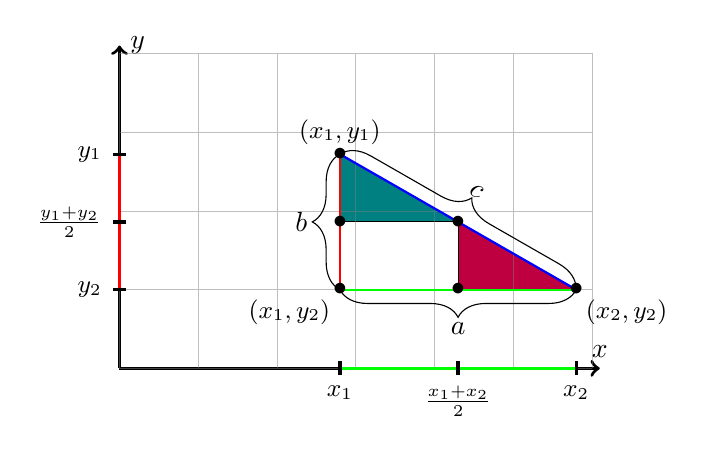
\begin{tikzpicture}
  \def\xmin{0}
  \def\xmax{6}
  \def\ymin{0}
  \def\ymax{4}

  \def\a{2.8}
  \def\b{2.72}
  \def\c{5.8}
  \def\d{1}
  \def\mx{{(\a + \c)/2}}
  \def\my{{(\b + \d)/2}}

  \coordinate (P) at (\a,\b);
  \coordinate (Q) at (\c,\d);
  \coordinate (R) at (\a,\d);
  \coordinate (MX) at (\mx,\d);
  \coordinate (MY) at (\a,\my);
  \coordinate (M) at (\mx,\my);

  \draw [fill=teal] (P) -- (MY) -- (M);
  \draw [fill=purple] (M) -- (MX) -- (Q);

  \draw [very thick,->] (\xmin,0) -- (\xmax+.1,0) node [anchor=south] {$x$};
  \draw [very thick,->] (0,\ymin) -- (0,\ymax+.1) node [anchor=west] {$y$};
  
  \path [draw, help lines, opacity=.5]  (\xmin,\ymin) grid (\xmax,\ymax);
  \draw [very thick, green] (\a,0) -- (\c,0);
  \draw [very thick, red] (0,\b) -- (0,\d);
  \draw [very thick] (\a,2.5pt) -- +(0,-5pt) node [anchor=north, font=\small] {$x_1$};
  \draw [very thick] (\c,2.5pt) -- +(0,-5pt) node [anchor=north, font=\small] {$x_2$};
  \draw [very thick] (\mx,2.5pt) -- +(0,-5pt) node [anchor=north, font=\small] {$\frac{x_1+x_2}{2}$};
  \draw [very thick] (2.5pt,\b) -- +(-5pt,0) node [anchor=east, font=\small] {$y_1$};
  \draw [very thick] (2.5pt,\d) -- +(-5pt,0) node [anchor=east, font=\small] {$y_2$};
  \draw [very thick] (2.5pt,\my) -- +(-5pt,0) node [anchor=east, font=\small] {$\frac{y_1 + y_2}{2}$};
  
  \draw [thick,blue] (P) -- (Q);
  \draw [thick,green] (Q) -- (R);
  \draw [thick,red] (R) -- (P);
  
  \node at (P) {$\bullet$};
  \node at (Q) {$\bullet$};
  \node at (R) {$\bullet$};
  \node at (MX) {$\bullet$};
  \node at (MY) {$\bullet$};
  \node at (M) {$\bullet$};
  
  \node [above, font=\small] at (P) {$(x_1,y_1)$};
  \node [below right, font=\small] at (Q) {$(x_2,y_2)$};
  \node [below left, font=\small] at (R) {$(x_1,y_2)$};
  \draw [decorate,decoration={brace,amplitude=10pt,mirror},xshift=-4pt,yshift=0pt] (P) -- (R) node [midway,xshift=-14pt] {$b$};
  \draw [decorate,decoration={brace,amplitude=10pt,mirror},xshift=-4pt,yshift=0pt] (R) -- (Q) node [midway,yshift=-14pt] {$a$};
  \draw [decorate,decoration={brace,amplitude=10pt},xshift=-4pt,yshift=0pt] (P) -- (Q) node [midway,above,sloped,yshift=7.2pt,xshift=.2pt] {$c$};
\end{tikzpicture}
